\section{Case study: \acf{AV} braking}
\label{sec:case}

%The research and development of safe \acp{AV} is a competitive topic. 
\ac{AV} are safety critical \acfp{CPS} as any faults in their operation can lead to accidents resulting in injuries or fatalities. 
%What constitutes a safe \ac{AV} and the design of these systems is a highly controversial topic. 
Unfortunately, such faults have already occurred.
For instance, both Tesla and Uber have had autonomous vehicle accidents~\cite{stewart_2018,coldewey_2018}.

It is difficult to build complete models of these scenarios, as \ac{AV} companies tend to produce or customise their own vehicles with their own proprietary hardware and software.
Nevertheless, in this paper, we use these unfortunate incidents as inspiration for a case study for this paper, where we examine one aspect of \ac{AV} control: the braking mechanism.
%, designed differently to each other competitor, and each company has its own, unique issues with the safety of these systems.
%Each time an incident with an \ac{AV} system occurs, it hits the news headlines.
%Recently, Tesla and Uber vehicles' fatal accidents have been making news.

%In this case study we 
%However, the \ac{AV} system in this paper was designed with only the braking aspect of \ac{AV} systems in mind. 
Here, we integrate a sensor package consisting of five cameras and a \ac{LiDAR} sensor. 
Each of the five cameras feeds into an \ac{ANN} ensemble~\cite{Maqsood2004} of CNNs, using the Darknet library~\cite{darknet13}.
These ensembles classify their input image and provide a confidence level for the classified image, before passing this information to the controller.
The controller \ac{ANN} is a \ac{MLP}, and decides the best course of action given the environment and the status of the vehicle itself. 
It then outputs controls to the vehicles actuators, which in our case are represented by an accelerator and a brake.
%Finally, the controller outputs are sent back to the vehicle, where the actuators are then updated accordingly.
%Here, the actuators for this system are the accelerator, which increases the speed of the vehicle; and the brakes, which slow down the vehicle.
A diagram of the \ac{AV} used in this system is shown in Figure~\ref{fig:av}. 
%\todo{Consider adding a figure showing the NN layout}

\begin{figure}[t]
	\centering
	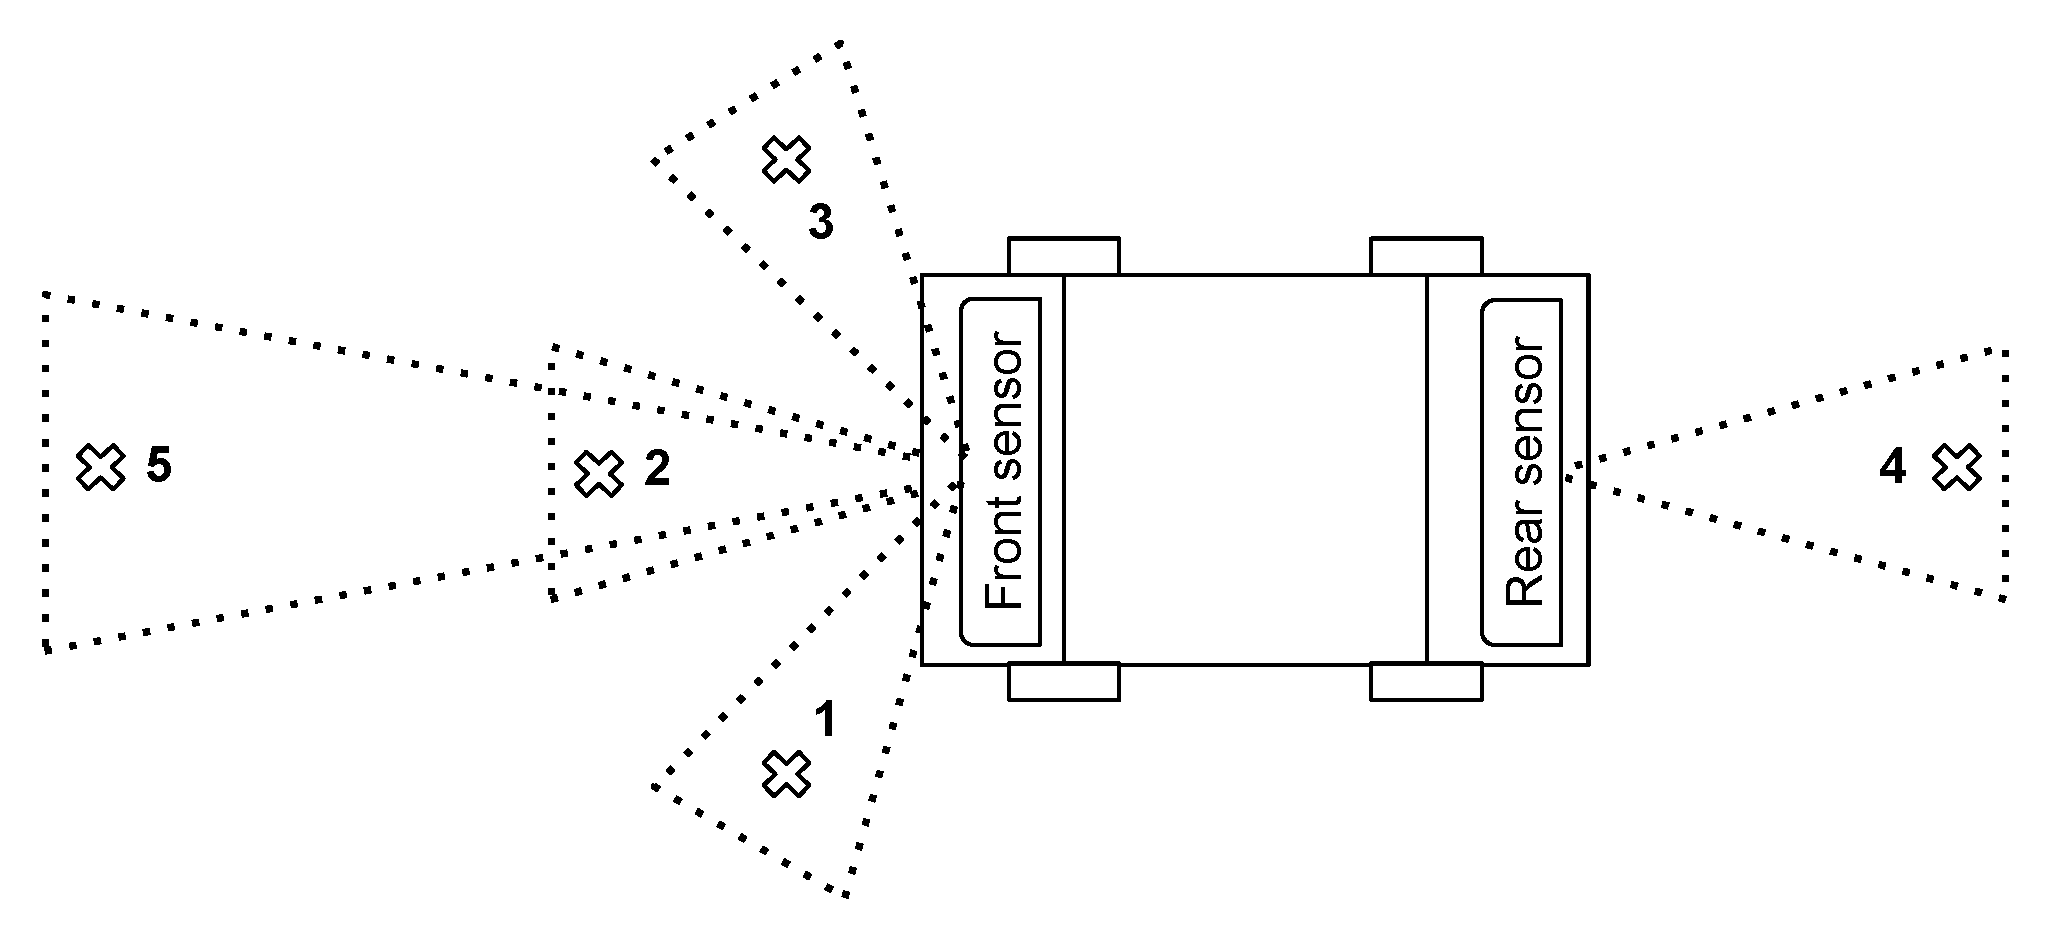
\includegraphics[width=\linewidth]{Content/fig/AV.pdf}
	\caption{Diagram showing the sensor layout for the \ac{AV}. \label{fig:av}}
\end{figure}

\begin{figure}[t]
	\centering
	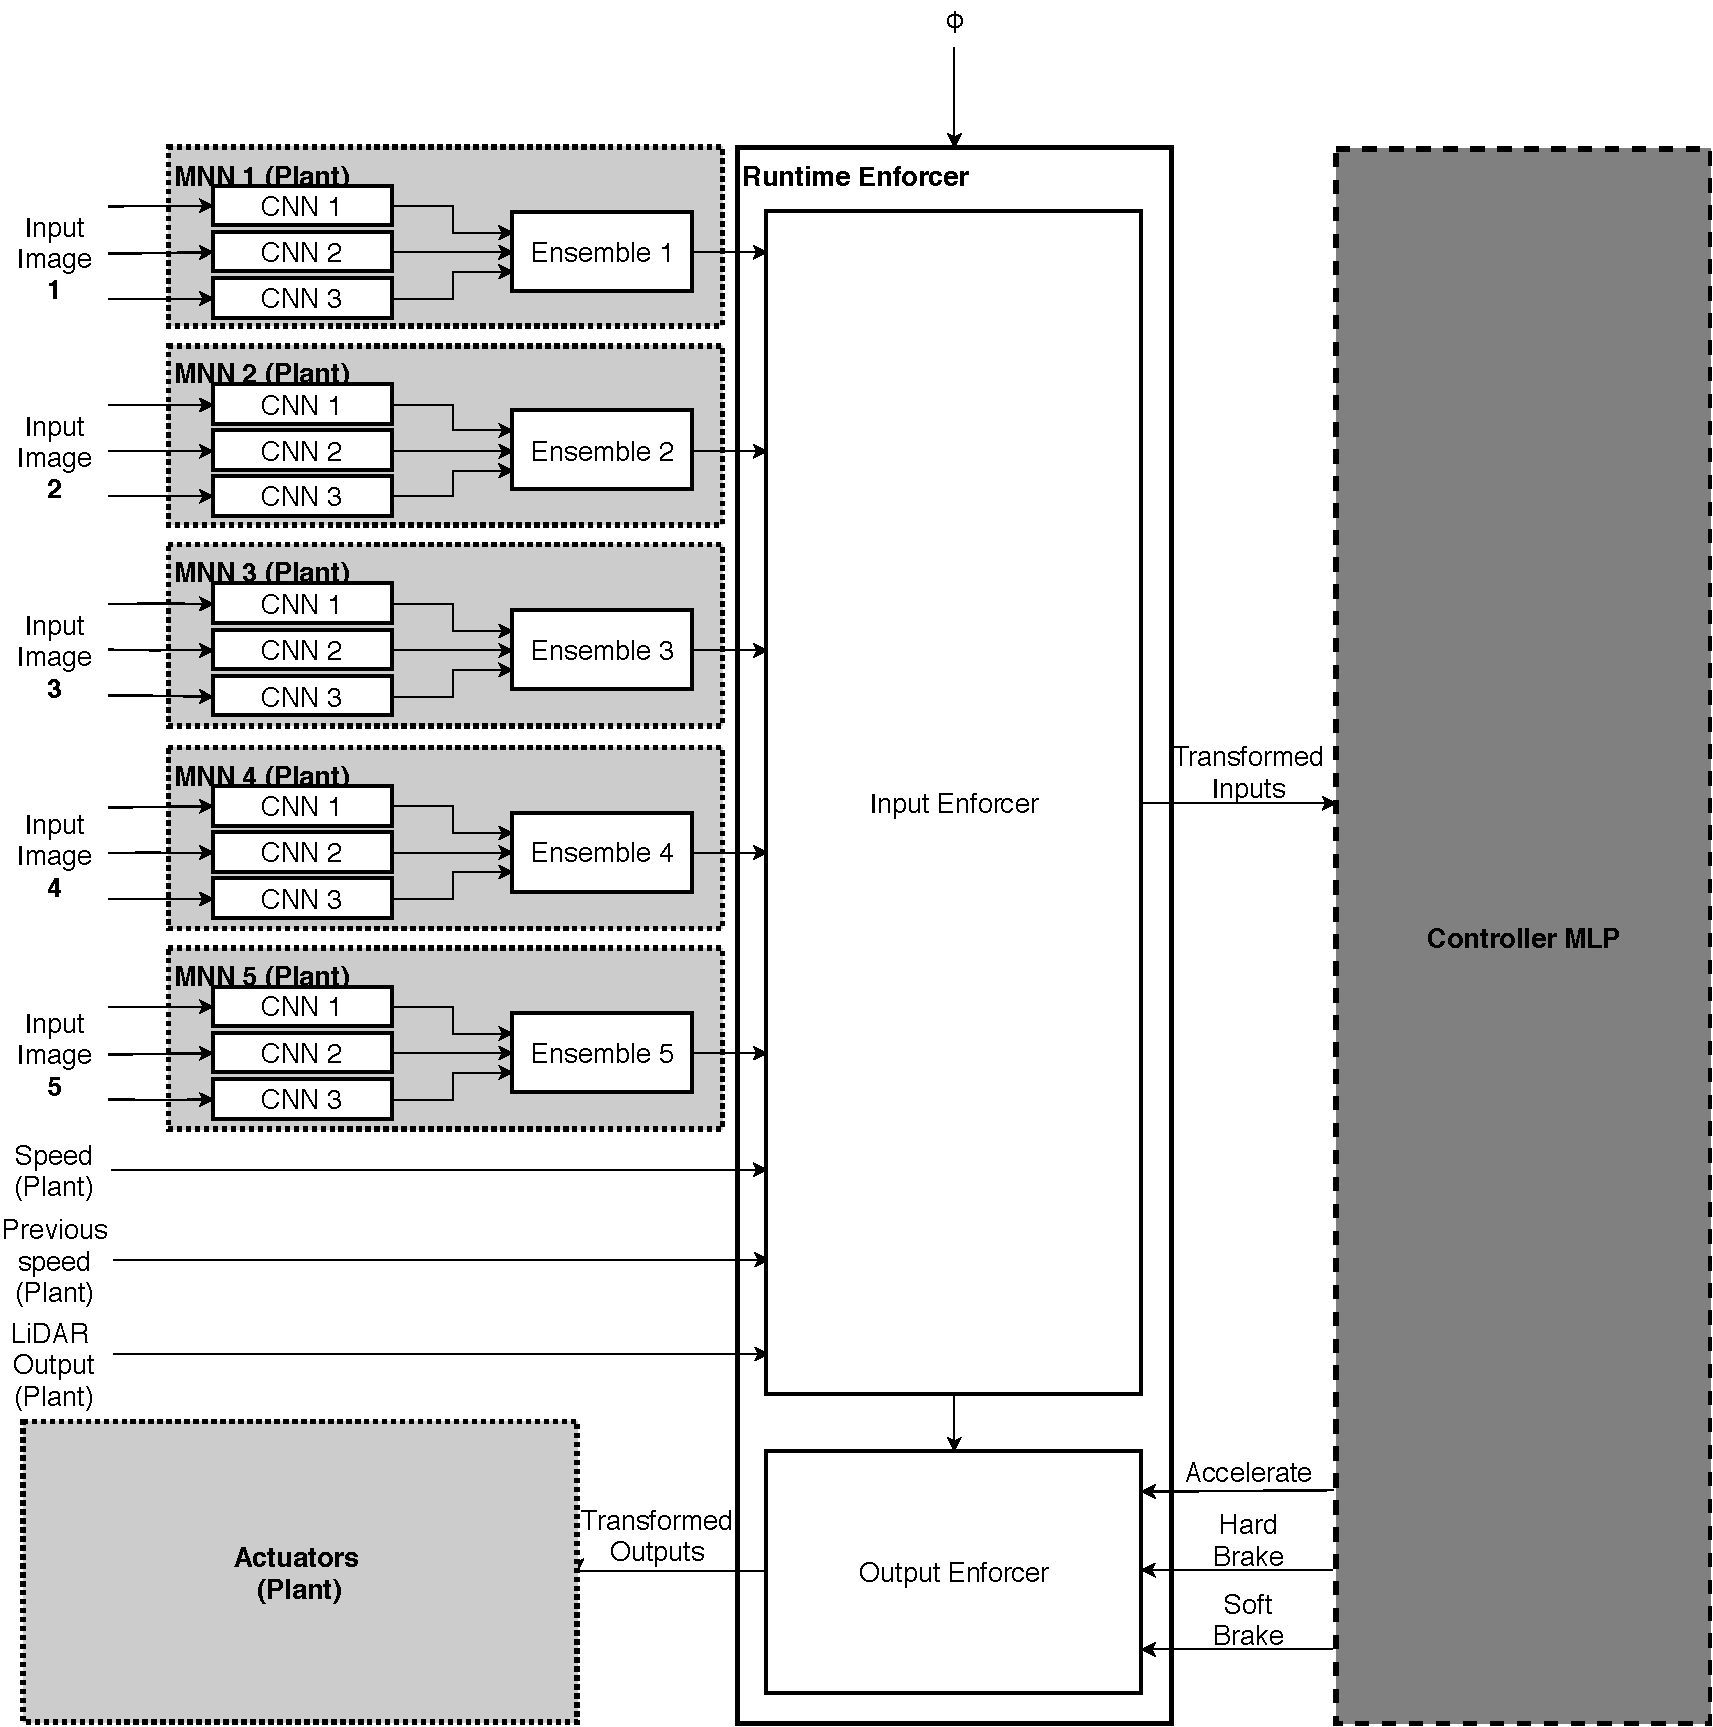
\includegraphics[width=\linewidth]{Content/fig/AV-MNN.pdf}
	\caption{Diagram showing the \ac{SNN} for the \ac{AV}. \label{fig:avmnn}}
\end{figure}

The controller \ac{MLP} takes seventeen different inputs. 
Two inputs correspond to the current speed of the vehicle ($S$) and the speed of the vehicle one tick in the past ($P$). 
The other fifteen inputs are broken into three boolean inputs for each camera's detected object ($O_1$ - $O_5$ as shown in Figure \ref{fig:av}): the type of object seen in that camera ($N$: nothing, $P$: pedestrian, $C$: car or $U$: unknown), the speed of the object ($V$) and the direction of the object ($D$).
E.g. a car far in-front of the \ac{AV} would be represented by $O_5$ as $O_{5_C}$, and its speed and direction by $O_{5_V}$ and $O_{5_D}$ respectively.
Depending on these inputs, the controller outputs three values  $A$: accelerate, $B_S$ soft brake, or $B_H$: hard brake.
These outputs can each be between 0 and 1.
If any of the values exceed 0.1, the highest valued action is chosen, otherwise the vehicle takes no action, i.e. it will continue at current speed (which could be zero).
The enforcer layout of the \ac{AV} system can be seen in Figure~\ref{fig:avmnn}.

Due to this design of this system, it is possible for the vehicle to behave badly in various ways. 
These include not driving at all, speeding, unnecessarily slamming the brakes, hitting other vehicles on the road and hitting pedestrians both on and off the road.
All of these scenarios can result in fatalities, thus classifying this system as a safety critical.
To have a system that is safe, policies need to be enforced that monitor the system's inputs and outputs and ensure that none of the above scenarios take place under any circumstances.
%This system is designed for two purposes: (1) to conceptualize \acp{SNN} and show their architecture; and (2) to show the efficacy of these \acp{SNN}.



\ac{RE} allows for easier formal reasoning over the possible runtime behaviour of the \acp{ANN} internal to the system, thus no longer requiring difficult static analysis.
\ac{RE} can apply a set of policies on the inputs and outputs of the system to ensure it follows a set of given constraints. % \acp{SANN} to ensure that the policies are never violated. 
These policies can also feature timing information to guarantee timing deadlines for real-time systems.
A well designed policy can thus ensure that the system never exhibits unsafe events --- therefore keeping the system's inputs and outputs \textit{safe}~\cite{EstSafeCriteria2003}. 

%However, these \ac{RE} models look at the enforced system as a black box. 
%For the purpose of \ac{RE} of an \ac{SANN} and its timed properties, the \ac{SANN} needs to be viewed as a white box, i.e. data internal to the \ac{SANN} needs to be able to be viewed and/or modified.
%Given that \acp{SANN} are white boxes, we develop white box \acp{SNN} that can include enforcers that are able to monitor the \ac{SANN} as white boxes.








